\documentclass[11pt]{beamer}
\usetheme{Warsaw}
\usepackage[utf8]{inputenc}
\usepackage[]{babel}
\usepackage{amsmath}
\usepackage{amsfonts}
\usepackage{amssymb}
\usepackage{graphicx}
\author{翁俊}
\title{Majoron 学习理解第一次汇报}
\usepackage{xeCJK}
\usepackage{ctex}
\usepackage{mathrsfs}
\usepackage{amsmath}
\usepackage{amsfonts}
\usepackage{amssymb}
\usepackage{siunitx}
\usepackage{float}
\usepackage{varioref}
\usepackage{cite}
\usepackage{hyperref}
\usepackage{amsmath}
 \usepackage{siunitx}
%\setbeamercovered{transparent} 
%\setbeamertemplate{navigation symbols}{} 
%\logo{} 
%\institute{} 
\date{} 
%\subject{} 
\begin{document}

\begin{frame}
\titlepage
\end{frame}

%\begin{frame}
%\tableofcontents
%\end{frame}

\begin{frame}{B-L自发破缺模型}
\begin{enumerate}
\item {Dirac 中微子:质量项保持了轻子数守恒。}
\item {Majorana 中微子:质量项破坏轻子数守恒
\begin{enumerate}
\item {引入右旋中微子Majorana质量项或轻子数耦合到Higgs场破坏轻子数守恒}
\item {轻子数守恒局部破缺,产生有质量的矢量介子,耦合到轻子流}
\item {轻子数守恒整体自发性破缺,产生无质量的Goldstone  boson}
\end{enumerate}
}
\end{enumerate}
第三种情况下的Goldstone boson 为Majoron(记作J),与物质的相互作用非常微弱,以至于在实验上很难看到。
\end{frame}

\begin{frame}{右手中微子模型中的Majoron}
自旋为0的规范单态场S与Yukawa耦合后:
$$
-\mathscr{L}_{Y}^{\prime}=\sum_{\ell, \ell^{\prime}} b_{\ell \ell^{\prime}} \overline{\widehat{N}}_{\ell L} N_{\ell^{\prime} \mathrm{R}} S+\text { h.c. }
$$
在标量势中,将B-L破坏的项去掉以后,B-L是global对称的。

S带有量子数,当真空期望值$<S>\neq 0$时,B-L对称性破缺,也就产生了Majoron。

S是复数形式的场,实部是其真空期望值,虚部则是Majoron。



\end{frame}

\begin{frame}{右手中微子模型中的Majoron}
一圈图如图:(计算方法还需要复习)
\begin{figure}[H]
 \centering
 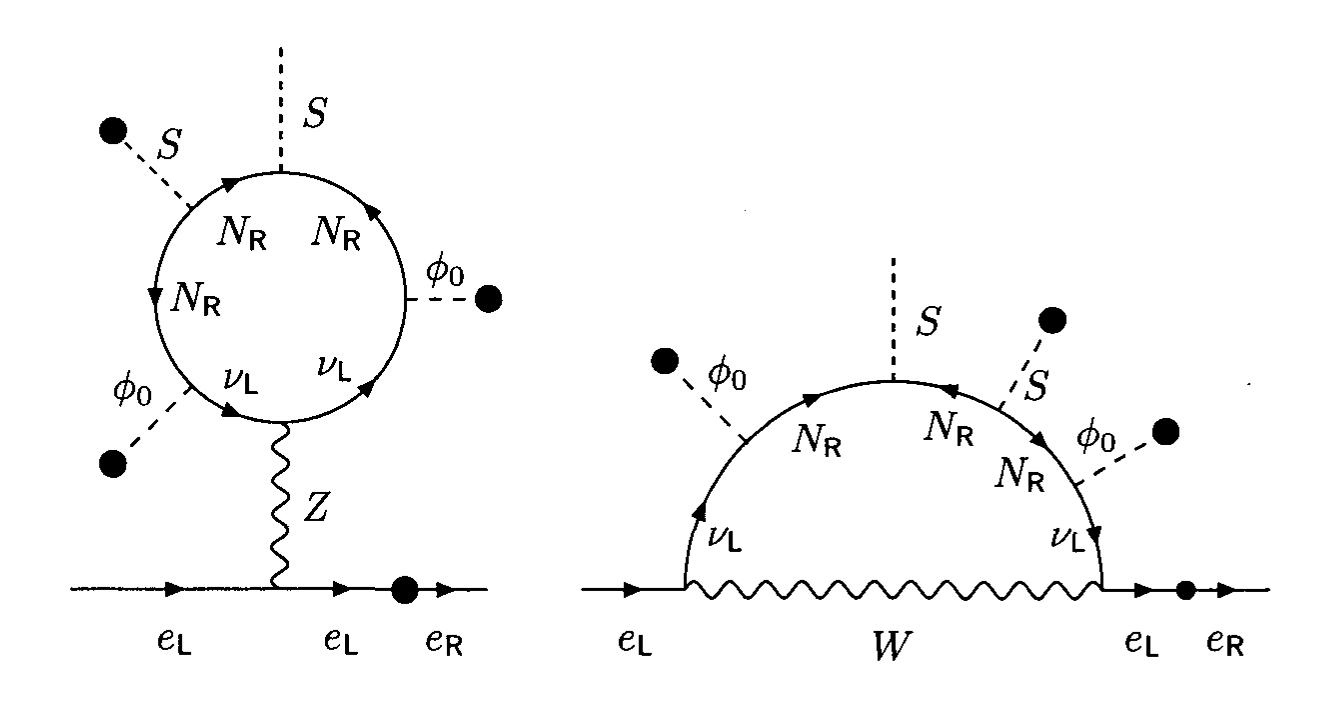
\includegraphics[height=4cm]{pic/1.png}
 \caption{Majoron与Fermion的耦合}
 \label{fig:1}
\end{figure}
计算得到Majoron与电子的耦合常数:
$$
g_{e J} \sim \frac{1}{16 \pi^{2}} G_{F} m_{e} \frac{M^{2}}{B} \sim \frac{1}{16 \pi^{2}} G_{F} m_{e} m_{\nu}
$$

\end{frame}

\begin{frame}{右手中微子模型中的Majoron}
在该模型下,存在如下过程:
$$
\nu \rightarrow \nu^{\prime}+J
$$
\begin{figure}[H]
 \centering
 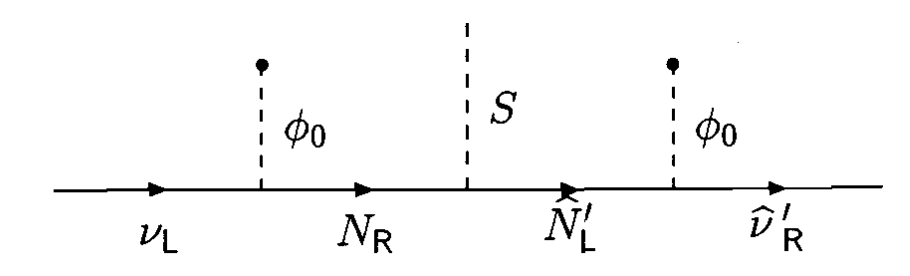
\includegraphics[height=2cm]{pic/2.png}
 \caption{中微子通过发射Majoron衰变}
 \label{fig:2}
\end{figure}
该过程的振幅与轻中微子和重中微子的混合比例的平方成正比,即为$\frac{M^2}{B^2}$,使得这个过程的寿命是大于宇宙寿命的。
\end{frame}

\begin{frame}{Majorons in models with extended Higgs sector}
这部分我还没有看完,下次一定
\end{frame}

\begin{frame}{Majoron观测的物理过程}
\begin{enumerate}
\item {$\mu \rightarrow e+J$
\begin{itemize}
\item {实验给出的衰变宽度:$\Gamma(\mu \rightarrow e+J)<3\times 10^{-4}$}
\item {类似的实验如kaons和pions衰变给出的结果比muon小两个数量级}
\item {目前给出限制:$g_{eJ}<10^{-10}$}
\end{itemize}}
\item {$\gamma+e \rightarrow e + J$
\begin{itemize}
\item {该过程是天体物理的观测范畴}
\item {Majoron发射到恒星外时,会携带能量,根据现有的恒星光度可给出限制}
\item {$
\sigma \simeq \frac{\left(e g_{e J}\right)^{2}}{12 \pi} \frac{\omega^{2}}{m_{e}^{4}};
L_{\mathrm{majo}} \simeq \frac{\alpha g_{e J}^{2} T^{6}}{3 m_{e}^{4} m_{p}}
$}
\item {目前给出限制:$g_{eJ}<10^{-10}$}
\end{itemize}
\begin{figure}[H]
 \centering
 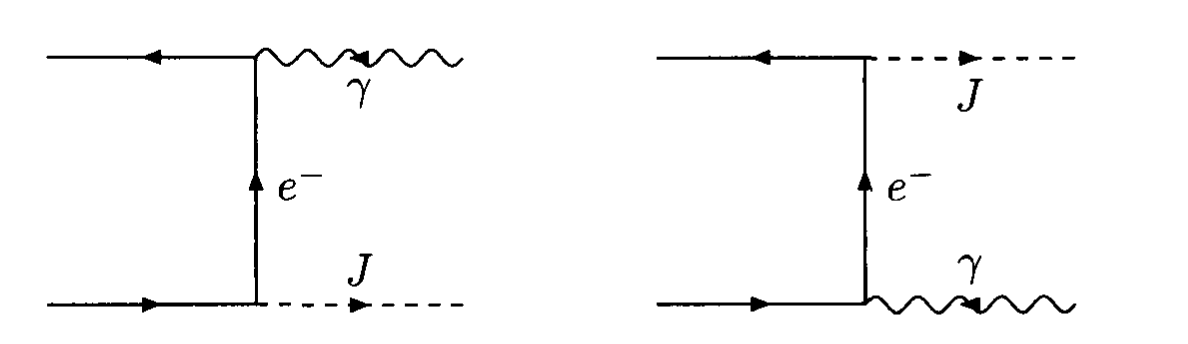
\includegraphics[height=2cm]{pic/3.png}
 \caption{Majoron的产生}
 \label{fig:2}
\end{figure}
}
\end{enumerate}
\end{frame}

\begin{frame}{下一步计划}
\begin{enumerate}
\item {中微子质量机制,不理解中微子质量机制,对于Majoron模型的理解会有囫囵吞枣的问题。}
\item {复习Feyman图计算(基本忘记完了)}
\item {Higgs机制,对于质量的理解,可能是必须的}
\item {JUNO实验,是否存在给出对Majoron发射过程$g_{eJ}$的更好限制的可能性。}
\item {。。。}
\end{enumerate}
\end{frame}
\end{document}